\documentclass[a4paper, 10pt]{scrartcl}

\usepackage{mathptmx} % more compact font
\usepackage[utf8]{inputenc}

\usepackage[english]{babel}
\usepackage{amsmath}
\usepackage{amsfonts}
\usepackage{mathtools}
\usepackage{multicol}
\usepackage{enumitem}
\usepackage{paralist} % for compacter lists
\usepackage{hyperref} % for Todo's and similar things
\usepackage[left=4.5mm, right=4.5mm, top=4.5mm, bottom=6mm, landscape, nohead, nofoot]{geometry}
\usepackage[small,compact]{titlesec}
\usepackage[extreme]{savetrees}
\usepackage[usenames,dvipsnames,svgnames,table]{xcolor}
\usepackage{xparse}
\usepackage{graphicx}
\usepackage{cancel}
\usepackage{dsfont}

% reinstate the Computer Modern calligraphic letters
\DeclareMathAlphabet{\mathcal}{OMS}{cmsy}{m}{n}

\setkomafont{section}{}
\setkomafont{subsection}{}
\setkomafont{subsubsection}{}
\setkomafont{paragraph}{\bfseries}
\setkomafont{subparagraph}{\mdseries}
\renewcommand{\familydefault}{\rmdefault}

% compact text
\linespread{0.9}
\setlength{\parindent}{0pt}

% compact lists even more
\setdefaultleftmargin{0em}{0em}{0em}{0em}{0em}{0em}

% compact sections
\titlespacing*{\section}{0pt}{0em}{0em}
\titlespacing*{\subsection}{0pt}{0em}{0em}
\titlespacing*{\subsubsection}{0pt}{0em}{0em}
\titlespacing*{\paragraph}{0pt}{0em}{5pt}
\titlespacing*{\subparagraph}{0pt}{0em}{4pt}

\newenvironment{talign*}
 {\let\displaystyle\textstyle\csname align*\endcsname}
 {\endalign}

% coloured section headings for easier read
\titleformat{name=\section}[block]
{\sffamily}
{}
{0pt}
{\colorsection}
\newcommand{\colorsection}[1]{%
	\colorbox{green!10}{\parbox[t][0em]{\dimexpr\columnwidth-2\fboxsep}{\thesection\ #1}}}

\titleformat{name=\subsection}[block]
{\sffamily}
{}
{0pt}
{\subcolorsection}
\newcommand{\subcolorsection}[1]{%
	\colorbox{lime!10}{\parbox[t][0em]{\dimexpr\columnwidth-2\fboxsep}{\thesubsection\ #1}}}


\titleformat{name=\subsubsection}[block]
{\sffamily}
{}
{0pt}
{\subsubcolorsection}
\newcommand{\subsubcolorsection}[1]{%
	\colorbox{lime!10}{\parbox[t][0em]{\dimexpr\columnwidth-2\fboxsep}{\thesubsubsection\ #1}}}

% environment for multicols inside a list
\NewDocumentEnvironment{listcols}{O{2} O{0pt}}
{%
	\bgroup %
	\setlength{\multicolsep}{#2} %
	\begin{multicols*}{#1} %
	}
	{%
	\end{multicols*} %
	\egroup %
}

% multicols lines & spacing
\setlength{\columnsep}{2mm}
\setlength{\columnseprule}{0.2pt}

% No page numbers
\pagenumbering{gobble}

% math helpers
\DeclareMathOperator*{\argmin}{arg\,min}
\DeclareMathOperator*{\argmax}{arg\,max}

\newcommand{\uP}{\mathrm P}

\begin{document}
\begin{centering}
\vspace*{1em}
\vfill
\textbf{Disclaimer} \\
We wrote this to our best knowledge, however, no guarantees are given whatsoever.
\vfill
\textbf{Sources} \\
If not noted differently, the source is the lecture slides and/or the accompanying book.
\vfill
\textbf{Contribute} \\
Please report errors and contribute back your improvements to the github repository at:
http://github.com/timethy/probabilistic\_ai \\
If you don't, may all your models overfit and your data be spoiled for ever.
\vfill
\end{centering}

\clearpage

	\begin{multicols*}{3}
		
		\defaultleftmargin{}{}{}{} 
		\section{Probabilities}
		\begin{talign*}
		\uP(A\mid B) & = \; \frac {\uP(B\mid A) \cdot \uP(A)} {\uP(B)} = \frac{\uP(A\cap B)}{\uP(B)} \\
		\uP(A, B) & = \uP(A \cap B) = \uP(A|B)\uP(B) = \uP(B|A)\uP(A) \\
		\uP(A\cup B) & =\uP(A)+\uP(B)-{{\uP(A\cap B)}} \\
		\uP (X_{1},\dots,X_{n}) & = \uP(X_{1})\,\uP(X_{2}| X_{1})\,\uP(X_{3}| X_{1},X_{2})\,\cdots\,\uP(X_{n} | X_{1},\dots,X_{n-1}) \\
		\uP(X,Y|Z) & = \uP(X|Y,Z)\uP(Y|Z) \\
		\uP(X=x) & = \sum_{y}\uP(X=x,Y=y)=\sum _{y}\uP(X=x\mid Y=y)\uP(Y=y)
		\end{talign*}
		Conditional independence: $X \perp Y | Z$ iff $\uP(X, Y| Z) = \uP(X|Z) \uP(Y|Z)$. \\
		If $\uP(Y|Z) > 0$ equivalent to $\uP(X|Z,Y) = \uP(X | Z)$
	
		\section{Bayes Network}
		\paragraph{Naive Bayes} Effects are conditionally independent given a cause.
		
		\paragraph{Bayesian network $(G,P)$:} DAG with cond.\ prob.\ dist.\ $\uP(X_s| Pa_{X_{s}})$.
		 $(G,P)$ defines joint distribution $\uP (X_{1:n}) = \prod_{i} \uP(X_i| Pa_{X_{i}})$  .
%		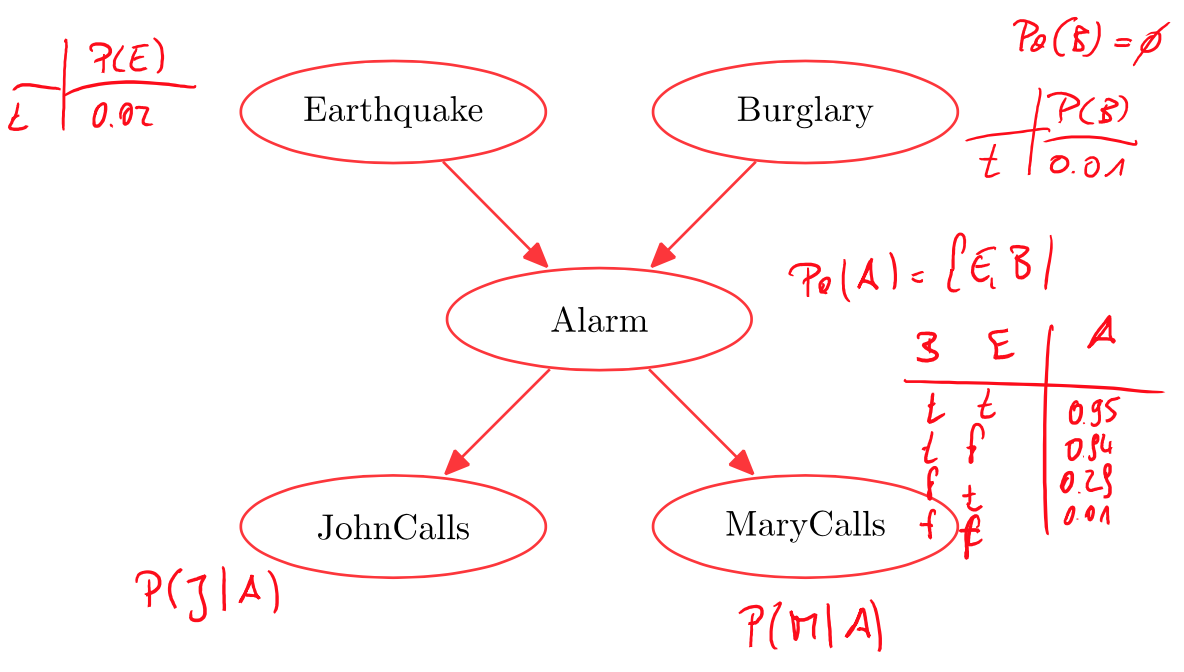
\includegraphics[height=2cm]{img/pai1.png}

		\paragraph{Specifying a BN}
		Variables $X_1, \cdots, X_n$. Pick order. For all $i \in [n]$ find 1.\ min.\ subset $A \subseteq \{X_1,\dots,X_{i-1}\}$ s.t.\ $X_i \perp X_{\bar A}|X_A$.
		2.\ Specify/learn $\uP(X_i|A)$.

		BN defined this way are sound. Ordering matters a lot for compactness of representation!
		
		\paragraph{Active Trails} If for all consecutive triplets $X, Y, Z$.
		\begin{compactitem}
			\item  $X \rightarrow  Y \rightarrow Z$ \& $Y$ is unobserved
			\item  $X \leftarrow  Y \leftarrow Z$ \& $Y$ is unobserved
			\item  $X \leftarrow  Y \rightarrow Z$ \& $Y$ is unobserved
			\item  $X \rightarrow  Y \leftarrow Z$ \& $Y$ or any of $Y's$ descendants is oberserved
		\end{compactitem}
	
		$A$ and $B$ \emph{d-seperated by $O$} iff no active trail exists with observations $O$.
		Implies c.i.: $\text{d-sep}(A;B | O) \Rightarrow A \perp B | O$.
		Algo for d-sep.: BFS
		
		\section{Inference}
		\paragraph{Typical Queries} Conditional Distribution, MPE ($\argmax_{e,b,a} \uP(e,b,a | J=t, M = f)$), MAP ($\argmax_{e} \uP(e | J=t, M = f)$)
		
		\subsection{Exact Inference}
		
		\paragraph{Variable Elimination}
		\begin{compactitem}
		\item Given BN and Query $\uP(Q | E=e)$ ($E$ = evidence variables)
		\item Choose an ordering of $X_1, ..., X_n$
		\item Set up initial factors: $fi = \uP(X_i | P_{ai})$
		\item For $i =1:n$, $X_i  \in X\setminus \{Q,E\}$
		\begin{compactenum}
			\item Collect and multiply all factors $f$ that include $X_i$  
			\item Generate new factor by marginalizing out $X_i$
			\item Add $g$ to set of factors, $g = \sum_{x_i}\prod_{j}f_j$
		\end{compactenum}
		\item  Renormalize $\uP(q,e)$ to get $\uP(q | e)$ = $\frac{1}{\sum_{q}\uP(q,e)}\uP(q,e)$
		
	\end{compactitem}

		
	\textbf{Variable Elimination for Polytrees}
	
	Polytree: A DAG is a polytree iff dropping edge directions results in a tree
	\begin{compactitem}
		\item Pick root
		\item Orient edges towards the root (only in this algo, not in actual BN)
		\item Eliminate in topological ordering (descendants before parents)
	\end{compactitem}

	\paragraph{Factor Graph}
	of BN is bipartite graph with variables on one side and factors on the other.
	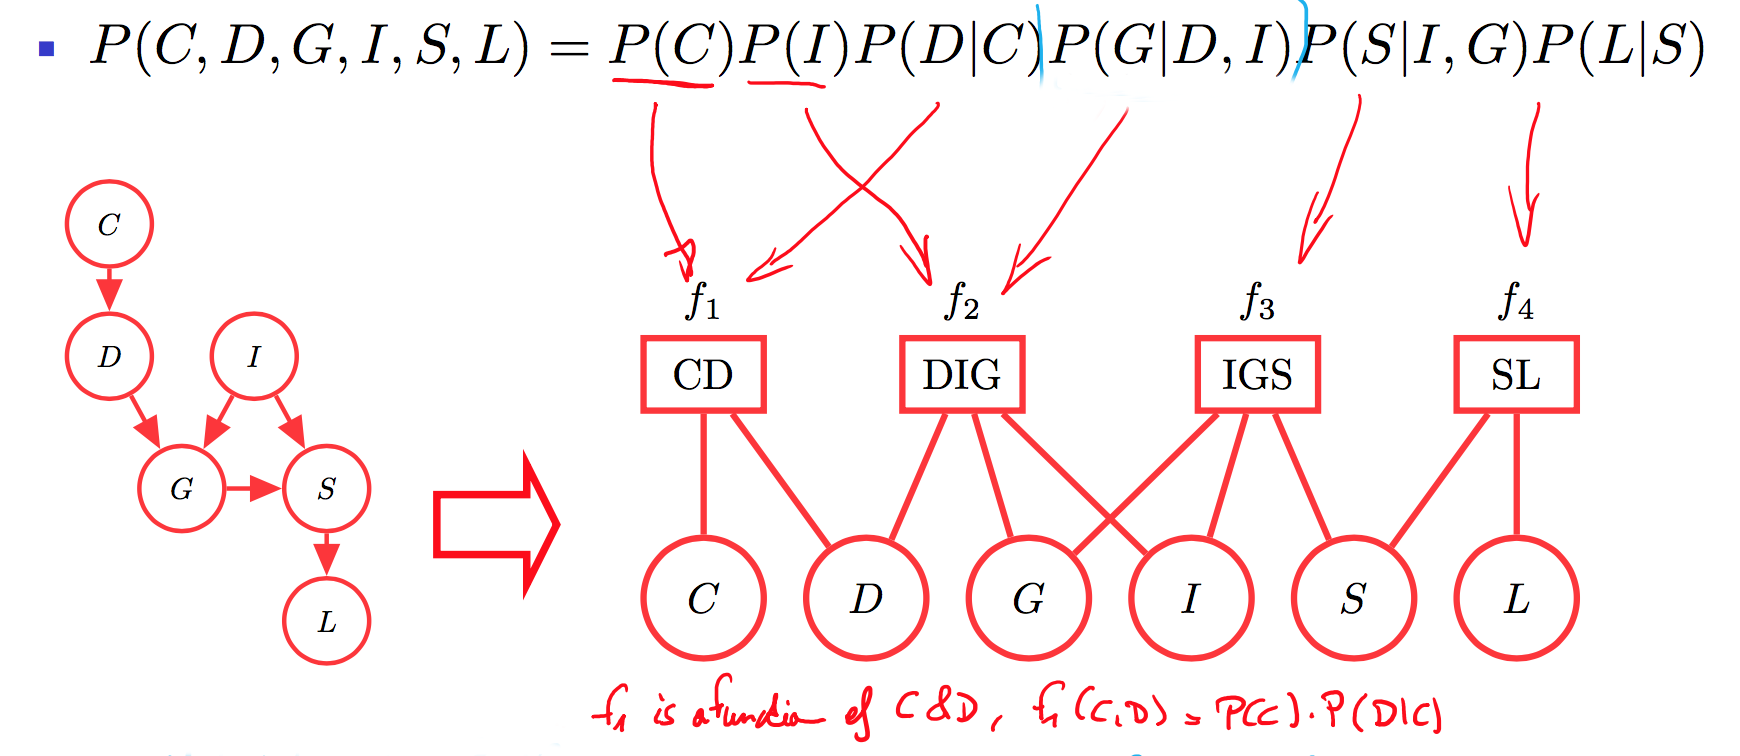
\includegraphics[height=2cm]{img/pai2.png}
	
	\paragraph{Sum-Product / Belief Propagation Algorithm}	
	
	\begin{compactitem}
		\item Initialize all messages as uniform distribution  
		\item Until converged do
		\begin{compactenum}
			\item Pick some ordering on the factor graph edges (+directions)   
			\item Update messages according to this ordering
			
			Messages from variable v to factor u: 
			
			$\mu^{(t+1)}_{v \rightarrow u}(x_v) = \prod_{u' \in N(v) \setminus \{u\}} \mu^{(t)}_{u' \rightarrow v}(x_{v})$ 
			
			Messages from factor u to variable v:
			
			$\mu^{(t+1)}_{u \rightarrow v}(x_v) = \sum_{x_u \sim x_v} f_u(x_u) \prod_{v' \in N(u) \setminus \{v\}} \mu^{(t)}_{v' \rightarrow u}(x_{v'})$ 

			\item Break once all messages change by at most $\epsilon$
		\end{compactenum}
	\end{compactitem}

	Intention: $\hat \uP(X_v = x_v) \propto \prod_{u \in N(v)} \mu_{u \rightarrow v} (x_v)$

	$\hat \uP(X_u = x_u) \propto f_u(x_u) \prod_{v \in N(u)} \mu_{v \rightarrow u} (x_u)$

	\paragraph{Belief Propagation on Trees (converges in two rounds)}
	\begin{compactitem}
		\item Factor graph of polytree is a tree!
		\item Choose one node as root
		\item Send messages from leaves to root, and from root to leaves
	\end{compactitem}
   
\paragraph{Variable Elimination for MPE}	
	\begin{compactitem}
	\item Given BN and evidence $E=e$
	\item Choose an ordering of $X_1,\dots,X_n$
	\item Set up initial factors: $f_i = \uP(X_i | Pa_i)$
	\item For $i=1:n, X_i \notin  E$
  	\begin{compactenum}
  	\item Collect and multiply all factors $f_j$ that include $X_i$   
  	\item Generate new factor by maximizing out $X_i, g_i = \max_{x_i} \prod_{j} f_j$
  	\item Add $g$ to set of factors
  	\end{compactenum}
	\item For $i=n:-1:1, X_i \notin  E$:  $\hat{x_i} = \argmax_{x_i} g_i(x_i, \hat{x}_{i+1:n})$
\end{compactitem}

\subparagraph{Example}
\begin{talign*}
  & \argmax_{e , b, a} \uP(e,b,a| J, M) = \argmax_{e, b, a} \bcancel{\frac{1}{Z}} \uP(e,b,a, J,M) \\
= & \argmax_{e , b, a} \uP(e)\uP(b)\uP(a|e,b)\uP(J|a)\uP(M|a) \\
= & \argmax_{a} \uP(J|a)\uP(M|a) \argmax_{e} \uP(e) \argmax_{b} \uP(b)\uP(a|e,b)
\end{talign*}
\begin{talign*}
a^{*} = &\argmax_{a} P(J|a)P(M|a) g_e(a) \\
e^{*} = &\argmax_{e} P(J|a^*)P(M|a^*) P(e) g_b(a^*,e)
\end{talign*}

\paragraph{Max-product Message Passing on Factor Graphs}

Messages from variable v to factor u: 

$\mu^{(t+1)}_{v \rightarrow u}(x_v) = \prod_{u' \in N(v) \setminus \{u\}} \mu^{(t)}_{u' \rightarrow v}(x_{v})$ 

Messages from factor u to variable v:

$\mu^{(t+1)}_{u \rightarrow v}(x_v) = \max_{x_u \sim x_v} f_u(x_u) \prod_{v' \in N(u) \setminus \{v\}} \mu^{(t)}_{v' \rightarrow u}(x_{v'})$ 
 
 \textbf{Retrieving MAP From Max-Product}
 \begin{compactitem}
 \item Define max-marginals: $P_{max}(X_v =x_v) = \max_{x \sim x_v} P(x)$
 \item For tree factor graphs, max-product computes max-marginals: 
 $P_{max}(X_v = x_v) \propto \prod_{u \in N(v)} \mu_{u \rightarrow v} (x_v)$ 
\item Can retrieve MAP solution from these (must be careful when ties need to be broken)
\end{compactitem}
\subsection{Approximate Inference}
Problem: if BN contains loops.
Loopy belief propagation will in general not converge	$\rightarrow$ Sampling Based Inference

\textbf{Monte Carlo Sampling from a BN (forward Sampling)}
\begin{compactitem}
	\item Sort variables in topological ordering $X_1,...,X_n$
	\item For $i=1$ to 	$n$ do: Sample $xi \sim P(X_i | X_1=x_1, ..., X_{i-1}=x_{i-1})$
\end{compactitem}

\textbf{Computing Probabilities Through Sampling}

Marginals: $P(w=t) \approx \frac{1}{N} \sum_{i=1}^{N}[w=t]x^{(i)} =\frac{ Count(w=t)}{N}$

Conditionals: $P(C=t | W=t) = \frac{P(C=t, W=t)}{P(w=t)} \approx \frac{Count(W=t, C=t)}{Count(W=t)}$

\textbf{Rejection Sampling}
``Normalen Würfel nehmen um Verteilung von 1..5 zu samplen, 6 wird jeweils ignoriert''

$\hat{P}(X_A = x_A | X_B = x_B) \approx \frac{Count(x_a, x_B)}{Count(x_B)}$

Throw away samples that disagree with $x_B$ problematic if $x_B$ is a rare event.

\paragraph{Markov Chain}

A Markov chain is sequence of RVs, $X_1,\dots,X_N$ with \emph{Prior} $\uP(X_1)$ \& \emph{transition probabilities} $\uP(X_{t+1} | X_t)$ independent of $t$.

\subparagraph{Ergodic:} $\exists t\in{\mathbb N}$ s.t. every state is reachable from every state in exactly $t$ steps.
Then it has unique, positive, stationary distribution.

$\exists$ unique stat. $\pi(x)>0\ s.t.\ \forall x \lim\limits_{N\rightarrow\infty}\uP(X_N = x)=\pi(x)$ indep. of $\uP(X_1)$.
\subparagraph{Ergodic Theorem:}$\lim\limits_{N\rightarrow\infty} \frac{1}{N}\sum_if(x_i)=\sum_{x\in D} \pi(x)f(x)$, where D finite state space.

\paragraph{Sampling from MC}
Sample $x_1 \sim \uP(X_1), x_2 \sim \uP(X_2 | X_1=x_1), \dots, x_N \sim \uP(X_N | X_{N-1}=x_{N-1})$.
If simulated “sufficiently long”, sample $X_N$ is drawn “very close” to the stationary dist.\ $\pi$.


\textbf{Gibbs Sampling: Random Order}
\begin{compactitem}
\item Start with initial assignment $x$ to all variables
\item Fix observed variables $X_B$ to their observed value $x_B$
\item For $t=1$ to $\infty$ do
\begin{compactenum}
\item Pick a variable $i$ uniformly at random from $\{1,..,n\} \setminus B$
\item Set $v_i = $values of all $x$ except $x_i$
\item Update $x_i$ by sampling from $\uP(X_i | v_i)$
\end{compactenum}
\end{compactitem}
Satisfies detailed balance equation! For unnormalized $Q$  $\forall x, x': \frac{1}{Z} Q(x)P(x'|x) = \frac{1}{Z} Q(x')P(x|x') $

\textbf{Gibbs Sampling: Practical Variant}
\begin{compactitem}
 \item Start with initial assignment $x^{(0)}$ to all variables
 \item Fix observed variables $X_B$ to their observed value $x_B$
 \item For $t=1$ to $\infty$ do 
\begin{compactenum}
\item Set $x^{(t)} = x^{(t-1)}$
\item For each variable $X_i$ (except those in $B$) 
\item Set $v_i =$ values of all $x^{(t)}$ except $x_i$
\item Sample $x_i^{(t)}$ from $\uP(X_i | v_i)$
\end{compactenum}
\end{compactitem}
No detailed balance, but also has correct stationary distribution.

\subparagraph{Ex.\ for Michi} $\uP(C|S,R,W=1) = \frac{\uP(C,S,R,W=1)}{\sum_{c'}\uP(C = c', S, R, W = 1)}$.

%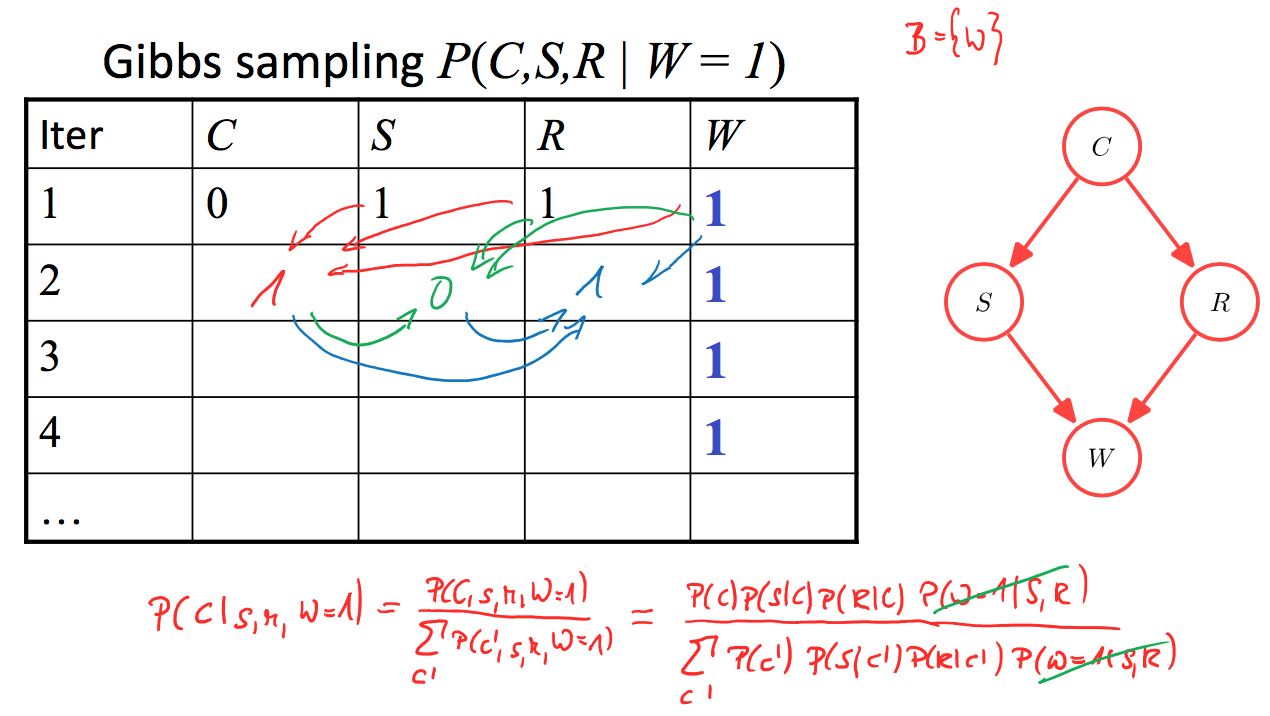
\includegraphics[height=2.5cm]{img/pai3.png}

\subsection{Temporal models}

\textbf{Markov Chains}

Markov assumption: $x_{t+1} \perp x_{1:t-1} | x_t \forall t$

Stationary asm.: $P(x_{t+1} = x | x_t = x') = P(x_{t'+1} | x_{t'} = x') \forall t, t'$

k-order: Next state depend on last k states.

\paragraph{Prediction in Markov Chains}
\begin{talign*}
\uP(X_i | X_1 = x) &= \sum_{x'}\uP(X_i,X_{i-1} = x'|X_1 = x) \\
 & = \sum_{x'}\uP(X_{i} | X_{i-1} = x', X_1 = x)\uP(X_{i-1} = x' | X_1 = x) \\
 & = \sum_{x'}\uP(X_{i} | X_{i-1} = x')\uP(X_{i-1} = x' | X_1 = x) \\
 & = f(\uP(X_{i-1}|X_1 = x)) = f^{i-1}(\uP(X_1 = x))
\end{talign*}

\paragraph{Hidden Markov Model/ Kalman Filters}

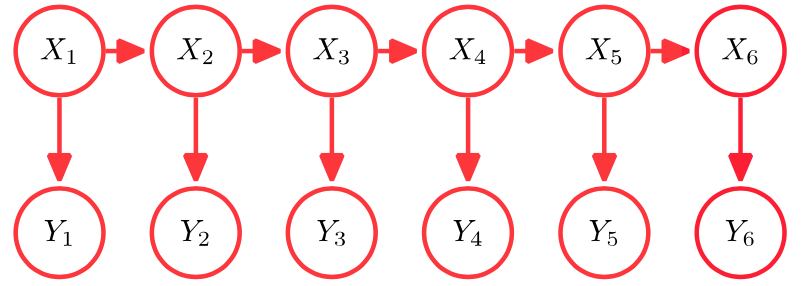
\includegraphics[height=1cm]{img/pai4.png}

$X_1,\dots,X_T$: Unobserved (hidden) variables (called states) \\
$Y_1,\dots,Y_T$: Observations \\
HMMs: $X_i$ categorical, $Y_i$ categorical (or arbitrary)\\
Kalman Filters: $X_i, Y_i$ Gaussian distributions

\paragraph{Inference Tasks}

Filtering: $P(X_t | y_{1:t} ) $; Prediction: $P(X_{t+T} | y_{1:t} )$ ; Smoothing: $P(X_t | y_{1:T}) \text{ for } 1\leq t < T$ ; MPE: $\argmax_{X_{1:T}} P(X_{1:T} | y_{1:T})$

In principle, can use variable elimination / belief propagation with new variables Xt, Yt at
each time step. Problem need to rerun every time, complexity grows with time!

\paragraph{Bayesian Filtering}
Suppose we already have computed $P(X_t | y_{1,\dots,t})$ now want to efficiently compute $P(X_{t+1} | y_{1,...,t+1})$

\begin{compactitem}
	\item Start with $P(X_1)$
	\item At time $t$ (Assume we have:  $P(X_t | y_{1,...,t-1})$
	\item Conditioning: $P(X_t | y_{y1:t}) = \frac{1}{Z} P(X_t | y_{1:t-1})P(y_t | X_t)$
	\item $Z= \sum P(x,y_t | y_{1:t-1})$
	\item Prediction: $P(X_{t+1} | y_{y1:t}) = \sum_{x_t}  P(X_t | y_{1:t}) P(X_{t+1} | x_t)$
\end{compactitem}
Computation is recursive (cost independent of t)!

\paragraph{Dynamic Bayesian Networks}
If we have more than one variable at each time step
\begin{compactitem}
	\item At every timestep have a replicated BN
	\item Variables at each time step $t$ called a slice $S_t$
	\item ``Temporal'' edges connecting $S_{t+1}$ with $S_t$ (usually sharing parameters -- stationarity)
	\item Can use standard approximate inference techniques (many loops) but high complexity over timesteps
\end{compactitem}

\paragraph{Particle filtering}
Approximate the posterior at each time by samples (particles), which are propagated and reweighted over time.
True distribution (possibly continuous): $P(x)$, $N$ i.i.d. samples: $x_1,..x_N$; Represent: $P(x) \approx \frac{1}{N} \sum_{i=1}^{N} \delta_{x_i}(x)$. E.g. $\delta_{x_i}(x):= x_i = x$

\begin{compactitem}
	\item Suppose $P(X_t | y_{1:t}) \approx \frac{1}{N} \sum_{i=1}^{N} \delta_{x_i, t}$ (measurement)
	\item Prediction: Propagate each particle: $x'_i \sim P(X_{t+1} | x_{i,t})$ (movement)
	\item Conditioning: Weigh particles: $w_i = \frac{1}{Z}P(y_{t+1} | x'_i)$
	\item Conditioning: Resample $N$ particles: $x_{i, t+1} \sim \frac{1}{N} \sum_{i=1}^{N} w_i\delta_{x'_i}$ 
\end{compactitem}

\subsection{Probabilistic planning}
How should we control the robot to maximize reward?

\paragraph{Markov Decision Process (MDP)} -- ``controlled Markov chain'':
States $X=\{1,...,n\}$, actions $A=\{1,...,m\}$, transition probabilities $\uP(x' | x, a) = \Pr[\text{next state } = x' | \text{Action } a \text{ in state } x)]$ and reward function $r(x,a, x')$.

\subparagraph{Modes} Finite horizon ($T$ timesteps) or discounted rewards ($\infty$ timesteps but discount factor $\gamma \in [0, 1)$).

\paragraph{Value of policy} deterministic (fixed) policy $\pi: X \rightarrow A$.
\begin{talign*}
V_\pi(x) & = J(\pi | X_0 = x) = \mathbb{E}[\sum_{t=0}^{\infty} \gamma^t r(X_t, \pi(X_t)) | X_0 = x] \\
         & = \sum_{x'}\uP(x'|x,\pi(x))[r(x,\pi(x),x')+\gamma V_\pi(x')]. \\
         & = r(x, \pi(x)) + \gamma \sum_{x'} \uP(x' | x, \pi(x)) V_\pi(x')
\end{talign*}
Given $\pi$, compute $V_\pi$ exactly by solving linear system!

\paragraph{Greedy policy}
\begin{talign*}
\pi_g(x) & = \argmax_a\sum_{x'}\uP(x'|x,a)\left(r(x,a,x')+\gamma V_\pi(x')\right) \\
         & = \argmax_a r(x,a) + \gamma\sum_{x'}\uP(x'|x,\pi(x))V_\pi(x')).
\end{talign*}

\paragraph{Bellmann Eq.}
Policy opt.\ $\iff$ greedy w.r.t.\ its induced value function. \\
$V^*(x) = \max_a\left[ r(x,a) + \gamma\sum_{x'}\uP(x'|x,a)V^*(x')\right]$.

%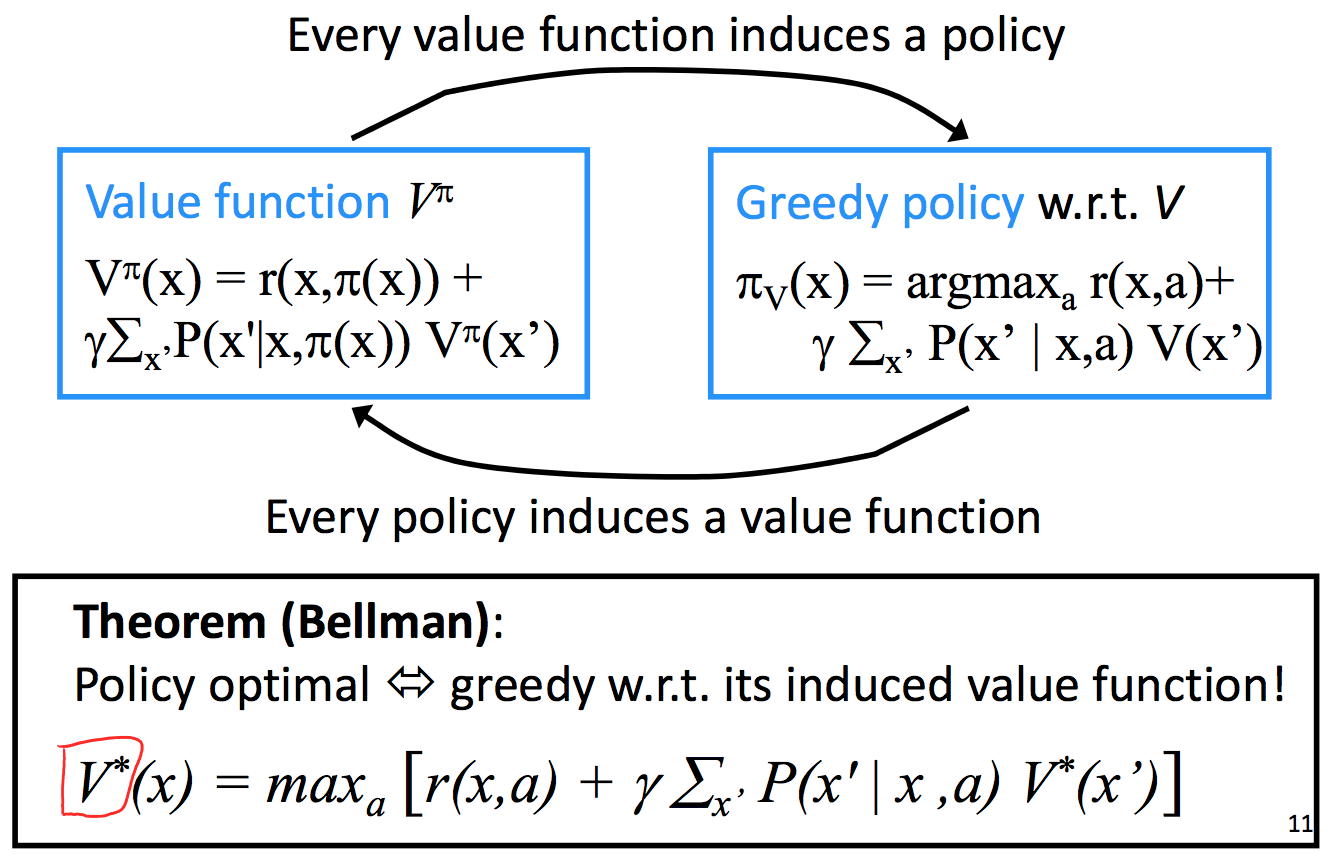
\includegraphics[height=3.5cm]{img/pai5.png}
\paragraph{Policy iteration}
Start with random (or smartly chosen) policy $\pi$.
Until convergence: State value function $V_\pi(x) \forall x$, solve linear system.
New policy is greedy policy $\pi \leftarrow \pi_G$ w.r.t.\ $V_\pi$.

Converged when $\pi = \pi_G$.
Guaranteed to monotonically improve, thus converging to an optimal policy in poly.\ steps.
Iteration: $O(n^3)$-time.

\paragraph{Value iteration}
Initialize $V_0(x) = \max_a r(x, a)$.
In time step $t$ until convergence:
\begin{talign*}
Q^t(x,a) & = r(x, a) + \gamma \sum_{x'} \uP(x' | x, a) V_{t-1}(x'), \forall x,a \\
V_t(x) & = \max_a Q^t(x,a), \forall x
\end{talign*}
Stop if $\max_x |V_t(x) - V_{t-1}(x)| < \epsilon$ else loop with greedy policy w.r.t.\ $V_t$.

Converges to $\epsilon$-optimal policy in polynomial steps. Iteration: $O(n\cdot m\cdot a)$-time. Not monotonically increasing.

\paragraph{Partially Observable MDP (POMDP)} ``controlled HMM''

Key idea: Interpret POMDP as an MDP with enlarged state space: New states correspond to beliefs $P(X_t | y_{1:t})$ in the original POMDP

\section{Learning BN}
Learn from i.i.d. data: 1.) Learning structure (conditional independencies) 2.) Learning parameters (CPDs)

\subsection{Parameter learning}
$P(X_1, ..., X_N) = \prod_{i=1}^{n} P(X_i | Pa_i, {\theta}_{i | Pa_i})$

Given:  BN structure $G$ \& Data set $D$ of complete observations
For each variable $X_i$ estimate: $\hat{\theta}_{X_i | Pa_i} = \frac{Count(X_i , Pa_i)}{Count(Pa_i)}$ (MLE)

We can also use a Beta prior (A priori knowledge) or simple regularization.

\subsection{Structure learning}
Score based structure learning: scoring function S(G;D). Quantifies, for each structure G the fit to the data D. 

$G^* = \argmax_G S(G;D)$; MLE: $S(G;D) = \max_\theta \log P(D | \theta, G)$

$\log P(D | \theta_{G \text{, MLE for G}}, G) = N \sum_{i=1}^{n} \hat{I}(X_i; Pa_i) + c$.

Problem: Optimal solution for MLE is always the fully  connected graph. 

\paragraph{Mutual Information (MI)}
$I(X_i; X_j) = \sum_{X_i, X_j} \uP(X_i, X_j) \log \frac{\uP(x_i, x_j)}{\uP(x_i) \uP(x_j)} \geq 0$
%(Def.\ analog.\ for sets $\mathbf{X}_A, \mathbf{X}_B$).

\subparagraph{Empirical MI}
$\hat{\uP}(X_i, X_j) = \frac{\#(X_i, X_j)}{N}$, $\hat I(X_i; X_j) = \sum_{x_i, x_j} \hat{\uP}(x_i, x_j) \log \frac{\hat{\uP}(x_i, x_j)}{\hat{\uP}(x_i) \hat{\uP}(x_j)}$

\subparagraph{Entropy}
$H(X_i) = -\sum_{x_i}\uP(x_i)\log\uP(x_i) = \mathbb{E}_{x_i}[-\log\uP(x_i)]$.

\subparagraph{Properties of MI}
$I(X_i; X_j) = 0$ iff $X_i, X_j$ independent. Symmetric.
$I(X_A; X_B) = H(X_A) - H(X_A|X_B)$.
$B \subseteq C \implies I(X_A; X_B) \leq I(X_A; X_C)$. %; proof: $I(X_A; X_B) = H(X_A) - H(X_A|X_B) \leq H(X_A) - H(X_A|X_C) = H(X_A)−H(X_A|X_C)=I(X_A;X_C)$

\paragraph{Bayesian Information Criterion (BIC)}
(Regularizing) $S_{BIC}(G) = \sum_{i=1}^{n} \hat{I}(X_i ; Pa_i) - \frac{\log N}{2N} |G|$ where $|G|$ is \# of parameters of G, n is \# of variables, N is \# of training examples.

``Haha this is now NP hard but finding optimal tree-shaped BN is possible''

\paragraph{Chow-Liu algorithm}
Given samples of $X_1,\dots,X_n$.
Find BN with exactly one parent per variable.
Gives opt.\ tree w.r.t.\ BIC.
\begin{compactitem}
	\item For each pair $X_i, X_j$ of variables compute $\hat{P}(x_i, x_j)$
	\item Compute Mutual Information $\hat{I}(X_i, X_j)$
	\item Take graph $K_n$, weight edge $(X_i,X_j) = \hat{I}(X_i, X_j)$
	\item Find maximum spanning tree of graph $\rightarrow$ undirected tree
	\item Pick any variable as root and orient the edges away using BFS
\end{compactitem}

\section{Reinforcement Learning}
``Learn mapping from (seq.\ of) actions to rewards''

\subsection{Passive Reinforcement}
Execute a set of trials in the environment using (fixed) policy  $\pi$
Reduction to a supervised problem. But does not exploit that values of states are not independent! (Bellman)

\subsection{Active Reinforcement Learning}
Not interested in fixed policy; need to decide action in every state. Fundamental Dilemma: Exploration-Exploitation.

\begin{compactitem}
	\item Always pick a random action - will eventually estimate all prob and rewards. May do extremely poorly. 
	\item Always pick the best action according to current knowledge - quickly get some rewards but can get stuck in suboptimal action.
\end{compactitem}

\subsubsection{Model-based RL }
Learn the MDP - optimize policy based on MDP.

\textbf{Learning the MDP}

Estimate transitions: $\hat{P}(X_{t+1} | X_t, A_t) = \frac{Count(X_{t+1}, X_t, A_t)}{Count(X_t, A_t)}$

Estimate rewards: $\hat{r}(X=x, A= a) = \frac{\sum_{t: x_t = x, a_t = a} r_t}{Count(X = x, A = a)}$

\textbf{ $\epsilon_t$ greedy}
With probability  $\epsilon_t$: Pick random action; With probability $(1- \epsilon_t)$: Pick best action

\paragraph{$R_{max}$ Algorithm}
Init: $r(x, a)$ = $R_{max}$.
$P(x^* | x, a) = 1$ where $x^*$ is a “fairy tale” state: $r(x^*, a) = r_{max}  \forall a$
Choose optimal $\pi$ according to $r$,$P$

Repeat:
Execute $Pi$. $\forall(x,a)\in visited$. update $r(x,a)$. Estimate $P(x'|x,a)$.
After "enough" rewards, recompute $\pi$ according to $r$,$P$.

Depends heavily on state space $O(|x|^3)$


\subsubsection{Model-free RL}
Estimate the value function directly.

\paragraph{Q-Learning}
$Q^*(x, a) = r(x, a) + \gamma \cdot \max_{a'} (Q^*(x', a'))$; $\gamma$ is discount factor.

\subparagraph{Algorithm} Init Q matrix to zero (or R if \emph{optimistic}).
\begin{compactitem}
	\item Select/Observe init state $x$
	\item Repeat until end state (restart after epoch):
	\item Select $a$ according to policy (i.e. $\epsilon$-greedy, or $\pi(x) = \argmax_a Q(x, a)$).
	\item Observe new state $x'$ and reward $r(x,a,x')$.
	\item $Q^{(t+1)}(x, a) \leftarrow (1-\alpha_t)Q^{(t)}(x, a) + \alpha_t(r(x,a,x') + \gamma \max_{a'}Q^{(t)}(x',a'))$
	\item $Q^{(t+1)}(x, a') \leftarrow Q^{(t)}(x, a') \forall a \neq a'$, remaining actions stay same.
	\item $Q^{(t+1)}(x'', a') \leftarrow Q^{(t)}(x'', a') \forall x'' \neq x$, remaining states stay same.
	\item $x \leftarrow x'$
\end{compactitem}

Depends on action space $O(|a|)$ (matrix size), i.e. iteration time is in $O(|a|)$.

\paragraph{Monte Carlo Tree Search (MCTS)}
Action selection planning
Simulate to terminal state observe reward and then propagate back result. Tree policies: epsilon greedy, random. Stop after sufficient runs or time budget.

\paragraph{Gradient Based Optimzation}
Objective Function: Mean Squared Value Error
Parameterize $V_\pi$ \& use SDG:
$\theta_{t+1} = \theta_{t} - \frac{1}{2}\cdot\alpha\nabla(V_\pi(s_t) - \hat{V}(s_t; \theta ))^2$
Can use Monte Carlo Estimate as surrogate for $V_\pi(s_t)$

\paragraph{Policy Gradient Method}
Learning a parameterized policy without the detour of learning a value function: $\pi(b) = \pi(b;\theta)$ \& again GD

\end{multicols*}
\end{document}


